% Provenance (never printed): see sources/outline_sources.md (Year 3:
% fractionation and Rayleigh distillation in the water cycle;
% palaeothermometry; carbon and sulfur isotopes). Brief:
% sources/book5/BRIEFS.md, ch. 14. Curves from figdata/bachelor-3/
% rayleigh_distillation.py, lr04_d18o.py, carbon_mass_balance.py. Exercise
% and problem values in the Book 5 scratch calculator calc/ch14.py. Dome Ilse,
% its traverse and the marine core are invented.
\chapter{Geoquímica de isótopos estáveis}\label{ch:b3:stable-isotopes}

A neve que cai sobre os domos elevados do manto de gelo da Antártida Oriental está entre
as águas mais leves da Terra. Cada uma de suas moléculas deixou o oceano na forma de vapor, e
no caminho para o interior, o ar perdeu a maior parte de sua água na forma de neve, primeiro as moléculas pesadas
O que resta na chegada depende de quanto foi perdido, o que por sua vez depende de
quão frio o ar ficou. Uma coluna de gelo é, portanto, um termômetro; uma concha
de calcita é outro, e o carbono dos calcários, um registro do que a
biosfera soterrou. Este capítulo deduz as leis por trás desses registros e
os interpreta.

\begin{recall}
O valor $\delta$, o fator de fracionamento $\alpha$ e os efeitos isotópicos de equilíbrio e
cinético estão nos volumes universitários dos livros de química. Os
padrões de referência VSMOW e VPDB e a reta meteórica estão no
volume do segundo ano, em seu capítulo sobre geoquímica de isótopos; a lei de
fracionamento de Rayleigh dos elementos-traço no capítulo sobre
diferenciação magmática; indicadores climáticos, o efeito de volume de gelo e o
termômetro Mg/Ca no capítulo sobre arquivos e indicadores climáticos; o
Máximo Térmico do Paleoceno--Eoceno no capítulo sobre clima ao longo do
tempo geológico; o Grande Evento de Oxidação no capítulo sobre a Terra pré-cambriana.
A fotossíntese e a redução bacteriana de sulfato estão nos livros de biologia.
\end{recall}

\section{Fracionamento entre duas fases}\label{sec:b3:stable-isotopes:fractionation}

Para duas fases A e B em equilíbrio isotópico, $\alpha_{A-B} = R_A/R_B =
(1000 + \delta_A)/(1000 + \delta_B)$, com as razões $R$ entre o isótopo pesado e o
isótopo leve. Vapor de água e água líquida têm $\alpha = 1.0098$ para o oxigênio-18
e $1.084$ para o deutério a \qty{20}{\celsius}, $1.0117$ e $1.111$ a
\qty{0}{\celsius}; gelo e água a \qty{0}{\celsius}, $1.0035$ e $1.0208$.
A fase mais pesada é sempre a mais condensada, e o fracionamento
cresce à medida que a temperatura cai.
% ledger: kc98:alpha, kc98:standards

\begin{definition}[Diferença isotópica]\label{def:b3:stable-isotopes:big-delta}
A \emph{diferença isotópica}\index{diferença isotópica (delta maiúsculo)}
entre duas fases é $\Delta_{A-B} = \delta_A - \delta_B$, em por mil.
\end{definition}

\begin{proposition}[A diferença isotópica e o fator de fracionamento]
\label{prop:b3:stable-isotopes:big-delta}
Para $\alpha$ próximo de 1 e valores pequenos de $\delta$,
\[
\Delta_{A-B} \approx 1000\ln\alpha_{A-B} \approx 1000(\alpha_{A-B} - 1).
\]
\end{proposition}

\begin{proof}
$1000\ln\alpha = 1000\ln(1 + \delta_A/1000) - 1000\ln(1 + \delta_B/1000)$, e
$1000\ln(1 + x/1000) = x - x^2/2000 + \dots$, logo $1000\ln\alpha = \delta_A -
\delta_B - (\delta_A^2 - \delta_B^2)/2000 + \dots$. Por fim, $\ln\alpha \approx
\alpha - 1$ para $\alpha$ próximo de 1.
\end{proof}

O erro é $(\delta_A^2 - \delta_B^2)/2000$: uma fração de um por mil nos
valores do oceano, quase um por mil entre o oceano e a neve leve do
gelo polar.
A grandeza $1000\ln\alpha$ é a que a teoria relaciona à temperatura: ela
varia quase com $1/T^2$ em altas temperaturas e com $1/T$ em baixas temperaturas,
e as calibrações são escritas nessa forma. Para o gelo e o vapor, por exemplo,
\[
\ln\alpha^{18}_{\mathrm{ice-v}} = \frac{11.839}{T} - 0.028224, \qquad
\ln\alpha^{\mathrm D}_{\mathrm{ice-v}} = \frac{16288}{T^2} - 0.0934,
\]
com $T$ em kelvins.
% ledger: gkinis14:alpha-ice, kc98:standards

\begin{definition}[Fracionamento dependente e independente da massa]\label{def:b3:stable-isotopes:mif}
Um elemento com três isótopos ou mais apresenta um \emph{fracionamento
dependente da massa}\index{fracionamento dependente da massa} quando os fracionamentos de
suas razões isotópicas estão na mesma proporção das diferenças de massa, como fixado pelas
massas; caso contrário, há um \emph{fracionamento independente
da massa}\index{fracionamento independente da massa}, medido pelo afastamento
da reta dependente da massa, como $\Delta^{33}\mathrm S = \delta^{33}\mathrm S
- 0.515\,\delta^{34}\mathrm S$.
\end{definition}

Para o oxigênio, o fracionamento de $^{17}\mathrm O/^{16}\mathrm O$ é cerca de 0.52 vez
o de $^{18}\mathrm O/^{16}\mathrm O$, valor próximo da razão entre as diferenças de massa, 1 para 2;
para o enxofre, $\delta^{33}\mathrm S = 0.515\,\delta^{34}\mathrm S$. O \omterm{def:b3:stable-isotopes:mif}{fracionamento independente
da massa} é raro: ocorre em meteoritos, no ozônio estratosférico e
no enxofre arqueano.
% ledger: white13c9:mdf, white13c9:s-mif

\section{Destilação de Rayleigh no ciclo da água}\label{sec:b3:stable-isotopes:rayleigh}

Uma massa de ar que resfria forma gotículas de nuvem ou cristais de neve, que caem e
saem. Cada condensado é mais rico em isótopos pesados do que o vapor, de modo que o
vapor restante fica mais leve, e o condensado seguinte, em equilíbrio com ele, é
também mais leve.

\begin{proposition}[Destilação de Rayleigh]\label{prop:b3:stable-isotopes:rayleigh-distillation}
Suponha-se que um reservatório de vapor perca sua água por condensados, cada um removido assim que
se forma em equilíbrio com o vapor. Se $f$ é a fração do
vapor restante e $\alpha$ o fator de fracionamento condensado--vapor, a
razão do vapor obedece a $\mathrm d\ln R_v = (\alpha - 1)\,\mathrm d\ln f$. Para
um $\alpha$ constante, tem-se a \emph{destilação de
Rayleigh}\index{destilação de Rayleigh}:
\[
\frac{R_v}{R_{v,0}} = f^{\,\alpha - 1}, \qquad
\delta_v = (1000 + \delta_{v,0})\,f^{\,\alpha - 1} - 1000,
\]
e o condensado formado em $f$ tem $\delta_c = \alpha(1000 + \delta_v) - 1000$.
\end{proposition}

\begin{proof}
Seja $N$ o número de moléculas de vapor (quase todas leves) e $N R_v$
o número das pesadas. Ao remover $\mathrm dN < 0$ moléculas de condensado
remove-se $\alpha R_v\,\mathrm dN$ pesadas: $\mathrm d(NR_v) = \alpha
R_v\,\mathrm dN$. Logo, $N\,\mathrm dR_v = (\alpha - 1)R_v\,\mathrm dN$, que é a
lei diferencial com $f = N/N_0$. Com $\alpha$ constante, integra-se em
uma lei de potência.
\end{proof}

Quando $\alpha$ depende da temperatura, $\ln(R_v/R_{v,0}) = \int(\alpha - 1)\,
\mathrm d\ln f$ ao longo do caminho. Para uma massa de ar resfriada a pressão constante,
a quantidade de vapor que ela pode reter é fixada pela pressão de saturação, logo $f =
e_s(T)/e_s(T_0)$, que a curva de sublimação do gelo fornece abaixo de
\qty{0}{\celsius}. A figura abaixo integra a lei para uma massa de ar cujo
vapor parte de \qty{0}{\celsius} com $\delta^{18}\mathrm O = -20$ admitido
e $\delta\mathrm D = \qty{-150}{\permil}$. O vapor real sobre o oceano é
mais leve do que o equilíbrio com a água do mar o tornaria, cerca de $-13$ em vez de
\qty{-9}{\permil} no oxigênio-18, porque a evaporação é em parte cinética.
% ledger: iapws:melt-subl, gkinis14:alpha-ice, white13c9:rayleigh

\begin{definition}[Excesso de deutério]\label{def:b3:stable-isotopes:d-excess}
O \emph{excesso de deutério}\index{excesso de deutério} de uma amostra de água é $d =
\delta\mathrm D - 8\,\delta^{18}\mathrm O$, em por mil.
\end{definition}

A precipitação dos continentes do Hemisfério Norte situa-se sobre a reta
$\delta\mathrm D = 8.0\,\delta^{18}\mathrm O + 10$: seu \omterm{def:b3:stable-isotopes:d-excess}{excesso de deutério} é de cerca de
\qty{10}{\permil}. A inclinação 8 está próxima da razão entre os fracionamentos de equilíbrio
dos dois isótopos na condensação. O excesso de 10, e não 0,
registra a evaporação cinética a partir do oceano, e o excesso de uma amostra
mede quão longe do equilíbrio a água da amostra evaporou.
% ledger: dansgaard64:effects, kc98:mwl

\begin{omfigure}
\begin{tikzpicture}
\begin{groupplot}[group style={group size=2 by 1, horizontal sep=1.6cm},
  omrecord, width=0.47\linewidth, height=0.42\linewidth, title style={font=\small},
  tick label style={font=\scriptsize}, label style={font=\small},
  legend style={font=\scriptsize, legend cell align=left}]
\nextgroupplot[title={(a) ao longo do caminho de resfriamento},
  xlabel={temperatura de condensação (\unit{\celsius})}, ylabel={$\delta^{18}\mathrm O$ (\unit{\permil})},
  xmin=-55, xmax=0, ymin=-130, ymax=0, x dir=reverse,
  legend style={at={(0.03,0.03)}, anchor=south west}]
% computed in figdata/bachelor-3/rayleigh_distillation.py
\addplot[omDef, thick, densely dashed] table[x=t, y=d18v] {figdata/out/bachelor-3-rayleigh_distillation-curve.dat};
\addlegendentry{vapor}
\addplot[omDef, thick] table[x=t, y=d18s] {figdata/out/bachelor-3-rayleigh_distillation-curve.dat};
\addlegendentry{neve}
\addplot[red!70!black, only marks, mark=*, mark size=1.6pt] table[x=t, y=d18s] {figdata/out/bachelor-3-rayleigh_distillation-stations.dat};
\addlegendentry{estações}
\nextgroupplot[title={(b) a neve no gráfico $\delta\mathrm D$--$\delta^{18}\mathrm O$},
  xlabel={$\delta^{18}\mathrm O$ (\unit{\permil})}, ylabel={$\delta\mathrm D$ (\unit{\permil})},
  xmin=-110, xmax=0, ymin=-700, ymax=0,
  legend style={at={(0.97,0.03)}, anchor=south east}]
\addplot[omDef, thick] table[x=d18s, y=dDs] {figdata/out/bachelor-3-rayleigh_distillation-curve.dat};
\addlegendentry{neve do modelo}
\addplot[black, densely dotted, domain=-110:0, samples=2] {8*x + 10};
\addlegendentry{$\delta\mathrm D = 8\,\delta^{18}\mathrm O + 10$}
\addplot[red!70!black, only marks, mark=*, mark size=1.6pt, forget plot] table[x=d18s, y=dDs] {figdata/out/bachelor-3-rayleigh_distillation-stations.dat};
\end{groupplot}
\end{tikzpicture}

\par\smallskip{\small \omterm{prop:b3:stable-isotopes:rayleigh-distillation}{Destilação de Rayleigh} de uma massa de ar resfriada a pressão constante
a partir de \qty{0}{\celsius}, com os fatores de fracionamento gelo--vapor
e a fração de vapor restante, lidos na curva de sublimação do gelo. (a) O
vapor (linha tracejada) e neve (linha contínua) ficam cada vez mais leves, cada vez mais rapidamente; os pontos são as
três estações do problema de fim de semana. (b) A neve do modelo permanece próxima da
reta meteórica até cerca de \qty{-30}{\permil} no oxigênio-18, depois sobe
acima dela.}\label{fig:b3:stable-isotopes:rayleigh}
\end{omfigure}
% ledger: kc98:mwl


\begin{definition}[Efeitos de temperatura, de quantidade e de continentalidade]\label{def:b3:stable-isotopes:effects}
O \emph{efeito de temperatura}\index{efeito de temperatura (isotópico)} é a
diminuição de $\delta^{18}\mathrm O$ e $\delta\mathrm D$ da precipitação com a
temperatura local. O \emph{efeito de quantidade}\index{efeito de quantidade} é a
diminuição desses valores com a quantidade de chuva, nos trópicos. O \emph{efeito de
continentalidade}\index{efeito de continentalidade} é a diminuição deles no interior do continente, a uma dada
temperatura.
\end{definition}

Os três são a \omterm{prop:b3:stable-isotopes:rayleigh-distillation}{destilação de Rayleigh} vista do solo. Em altas latitudes
o \omterm{def:b3:stable-isotopes:effects}{efeito de temperatura} domina: as médias anuais das estações da Groenlândia e do
Atlântico Norte seguem $\delta^{18}\mathrm O = 0.69\,t - 13.6$ e $\delta\mathrm D =
5.6\,t - 100$ (em por mil, com $t$ a temperatura média anual da superfície em
\unit{\celsius}). Nos trópicos domina o \omterm{def:b3:stable-isotopes:effects}{efeito de quantidade}: em uma ilha oceânica,
a chuva mensal perde cerca de \qty{1.6}{\permil} de oxigênio-18 a cada
\qty{100}{mm} a mais de chuva. O modelo simples da figura acima dá uma inclinação mais
acentuada, de cerca de \qty{1.6}{\permil} por grau de temperatura de condensação.
As inclinações não são diretamente comparáveis: a superfície de um manto de gelo é mais fria
do que o ar onde a neve se forma, e o modelo ignora a mistura de massas de ar
e os efeitos cinéticos da formação de neve, de modo que a inclinação em relação à
temperatura da superfície é calibrada, não calculada.
% ledger: dansgaard64:effects

\section{Paleotermometria}\label{sec:b3:stable-isotopes:palaeothermometry}

\begin{definition}[Paleotermometria, equação de paleotemperatura]
\label{def:b3:stable-isotopes:palaeothermometry}
A \emph{paleotermometria}\index{paleotermometria} é a medição de temperaturas passadas a partir da
composição de materiais formados então. Uma
\emph{equação de paleotemperatura}\index{equação de paleotemperatura} é uma
relação calibrada entre a temperatura de formação de um mineral e seu
fracionamento com a água a partir da qual ele cresceu.
\end{definition}

Para a calcita precipitada lentamente a partir da água, uma calibração fornece
\[
1000\ln\alpha_{\mathrm{calcite-water}} = 18.03\,\frac{10^3}{T} - 32.42,
\]
com ambos os valores de $\delta$ na escala VSMOW. Os carbonatos são expressos na
escala VPDB, convertidos pela relação $\delta^{18}\mathrm O_{\mathrm{VPDB}} =
0.97001\,\delta^{18}\mathrm O_{\mathrm{VSMOW}} - 29.99$. Perto de \qty{5}{\celsius} o
fracionamento cai cerca de \qty{0.23}{\permil} por grau de aquecimento.
% ledger: isogeochem:ko97

\begin{method}[Uma paleotemperatura de carbonato]\label{met:b3:stable-isotopes:palaeotemperature}
\begin{enumerate}
\item converta o $\delta^{18}\mathrm O$ da calcita de VPDB para VSMOW;
\item estime o $\delta^{18}\mathrm O$ da água a partir da qual a concha cresceu, na
escala VSMOW, corrigindo o valor atual pelo volume de gelo da época;
\item calcule $1000\ln\alpha = 1000\ln[(1000 + \delta_c)/(1000 + \delta_w)]$;
\item inverta a calibração: $T = 18.03\times10^3/(1000\ln\alpha + 32.42)$.
\end{enumerate}
\end{method}

A segunda etapa é a difícil. Durante uma glaciação, os mantos de gelo
armazenam água leve, e o oceano fica mais pesado. Cada metro de nível do mar corresponde
a cerca de \qty{0.011}{\permil} no $\delta^{18}\mathrm O$ do oceano; o último glacial
rebaixou o nível do mar em cerca de \qty{125}{m}, o que tornou o oceano cerca de
\qty{1.4}{\permil} mais pesado. Os organismos acrescentam deslocamentos próprios, os
efeitos vitais, e uma concha pode trocar oxigênio com a água intersticial após o soterramento.
% ledger: white13c9:ice-volume

\begin{omfigure}
\begin{tikzpicture}
\begin{axis}[omrecord, width=0.8\linewidth, height=0.32\linewidth, clip=false,
  xlabel={idade (\unit{\ka})}, ylabel={$\delta^{18}\mathrm O$ bentônico (\unit{\permil})},
  xmin=0, xmax=800, ymin=2.8, ymax=5.4, y dir=reverse,
  xtick={0,100,200,300,400,500,600,700,800},
  tick label style={font=\scriptsize}, label style={font=\small}]
% computed in figdata/bachelor-3/lr04_d18o.py from data/derived/lr04.csv
\addplot[omDef, thin] table[x=age_ka, y=d18O] {figdata/out/bachelor-3-lr04_d18o-stack.dat};
\draw[densely dotted] (axis cs:0,3.25) -- (axis cs:830,3.25);
\draw[densely dotted] (axis cs:20,5.02) -- (axis cs:830,5.02);
\draw[red!70!black, thick, |-|] (axis cs:830,3.25) -- node[right, font=\scriptsize, align=left] {volume de gelo\\\qty{1.4}{\permil}} (axis cs:830,4.625);
\draw[black, thick, |-|] (axis cs:830,4.625) -- node[right, font=\scriptsize] {resfriamento} (axis cs:830,5.02);
\end{axis}
\end{tikzpicture}

\par\smallskip{\small A pilha global de foraminíferos bentônicos $\delta^{18}\mathrm O$
nos últimos \qty{800}{\ka}, com o eixo invertido para que os tempos glaciais frios
fiquem embaixo. Do presente (\qty{3.25}{\permil}) até o último máximo glacial
(\qty{5.02}{\permil}), cerca de \qty{1.4}{\permil} da variação é o
volume de gelo (barra vermelha, à direita); o restante é um resfriamento da água profunda (barra
preta).}\label{fig:b3:stable-isotopes:lr04}
\end{omfigure}
% ledger: data:lr04, white13c9:ice-volume

\begin{definition}[Isótopos agrupados]\label{def:b3:stable-isotopes:clumped}
Os \emph{isótopos agrupados}\index{isótopos agrupados} são moléculas ou grupos que
contêm dois isótopos pesados ligados entre si. Em carbonatos, $\Delta_{47}$ é
o excesso, em por mil, da abundância de $^{13}\mathrm C^{18}\mathrm O^{16}\mathrm O_2$
grupos, medidos como dióxido de carbono de massa 47, em relação a uma distribuição
aleatória dos isótopos.
\end{definition}

Os isótopos pesados se ligam entre si um pouco mais do que o acaso permitiria,
e tanto mais quanto mais fria for a cristalização. O excesso depende apenas da
temperatura de crescimento, e não da composição da água: uma calibração unificada
é $\Delta_{47} = 0.0391\times10^6/T^2 + 0.154$ (em por mil, com $T$
em kelvins) de 0.5 a \qty{1100}{\celsius}. Medido junto com
$\delta^{18}\mathrm O$, ele fornece tanto a temperatura quanto a composição da
água. Sua sensibilidade é pequena, cerca de \qty{0.003}{\permil} por grau perto
de \qty{20}{\celsius}, o que exige medições longas.
% ledger: isogeochem:d47

\section{Isótopos de carbono}\label{sec:b3:stable-isotopes:carbon}

A fotossíntese fraciona o carbono cineticamente. A difusão do
dióxido de carbono para dentro de uma folha custa cerca de \qty{-4.4}{\permil}, a enzima RuBisCO
\qty{-29.4}{\permil}; as plantas da via comum C3 terminam \num{20} a
\qty{30}{\permil} mais leves do que o ar, e têm em média cerca de
\qty{-27}{\permil}, enquanto as da via C4 têm cerca de \qty{-13}{\permil}. O
carbono é leve, e o carbono inorgânico do qual ele é formado fica mais pesado.
% ledger: white13c9:photosynthesis, white:d13c

\begin{definition}[Fração de soterramento de carbono orgânico]\label{def:b3:stable-isotopes:forg}
A \emph{fração de soterramento de carbono orgânico}\index{fração de soterramento de carbono orgânico}
$f_{\mathrm{org}}$ é a fração do carbono que deixa o oceano e a
atmosfera, e é soterrada como matéria orgânica, em vez de como carbonato.
\end{definition}

\begin{proposition}[Balanço de massa dos isótopos de carbono]\label{prop:b3:stable-isotopes:forg}
Em estado estacionário, com entradas de composição $\delta_{\mathrm{in}}$ e soterramento de
carbonato $\delta_{\mathrm{carb}}$ e de carbono orgânico $\delta_{\mathrm{org}} =
\delta_{\mathrm{carb}} + \Delta_B$, o \emph{balanço de massa dos isótopos de
carbono}\index{balanço de massa dos isótopos de carbono} é
\[
\delta_{\mathrm{in}} = f_{\mathrm{org}}\,\delta_{\mathrm{org}} + (1 - f_{\mathrm{org}})\,
\delta_{\mathrm{carb}}, \qquad f_{\mathrm{org}} = \frac{\delta_{\mathrm{in}} -
\delta_{\mathrm{carb}}}{\Delta_B}.
\]
\end{proposition}

\begin{proof}
Em estado estacionário, o carbono que entra é igual ao carbono soterrado, e o
mesmo vale para o carbono-13; com valores de $\delta$, o balanço do carbono-13
é uma média ponderada pela massa dos valores de $\delta$, na aproximação
da \cref{prop:b3:stable-isotopes:big-delta}. Substituindo $\delta_{\mathrm{org}} =
\delta_{\mathrm{carb}} + \Delta_B$ e isolando, obtém-se $f_{\mathrm{org}}$.
\end{proof}

As entradas, provenientes de vulcões e do intemperismo de carbonatos antigos e
de matéria orgânica, são tomadas em cerca de \qty{-5}{\permil}, o valor do manto; $\Delta_B$
permaneceu entre $-32$ e \qty{-25}{\permil}; e os carbonatos mantiveram um
$\delta^{13}\mathrm C$ próximo de 0, dentro de cerca de \qty{1}{\permil}, ao longo da maior
parte da história da Terra. O balanço fornece então o clássico $f_{\mathrm{org}} \approx
0.2$: um quinto do carbono é soterrado como matéria orgânica e, com ele, o
oxigênio liberado pela fotossíntese permanece no ar. Trabalhos recentes argumentam que
$f_{\mathrm{org}}$ variou mais do que sugere essa constância.
% ledger: planavsky22:forg

\begin{definition}[Excursão isotópica do carbono]\label{def:b3:stable-isotopes:cie}
Uma \emph{excursão isotópica do carbono}\index{excursão isotópica do carbono} é uma
variação geologicamente breve do $\delta^{13}\mathrm C$ de carbonatos e de matéria
orgânica em todo o mundo, seguida de um retorno, registrada em seções sedimentares.
\end{definition}

\begin{proposition}[Massa de uma excursão]\label{prop:b3:stable-isotopes:cie-mass}
Carbono de composição $\delta_s$ e massa $m$, misturado a um reservatório trocável
de massa $M$ e composição $\delta_0$, desloca-o de $\Delta$ quando
\[
m = M\,\frac{\Delta}{\delta_s - \delta_0 - \Delta}.
\]
\end{proposition}

\begin{proof}
A mistura tem $(M + m)(\delta_0 + \Delta) = M\delta_0 + m\delta_s$, linear em
$m$.
\end{proof}

No início do Máximo Térmico do Paleoceno–Eoceno, entre 55.5 e
\qty{56.3}{\Ma}, o carbono do oceano e da atmosfera caiu de 2.5 para
\qty{4.0}{\permil} em menos de \qty{60}{kyr}. O carbono necessário é de cerca de
2000 a \qty{3500}{Gt} se era metano a \qty{-60}{\permil}, 6000 a
\qty{12000}{Gt} se era carbono orgânico a \qty{-25}{\permil}: quanto mais leve
a fonte, menos carbono é necessário. Lidas de trás para frente, com a proposição
e $\delta_0 = 0$, essas estimativas implicam um reservatório trocável de \num{46000}
a \qty{63000}{Gt} de carbono.
% ledger: dickens11:petm

\begin{omfigure}
\begin{tikzpicture}
\begin{groupplot}[group style={group size=2 by 1, horizontal sep=1.7cm},
  omrecord, width=0.47\linewidth, height=0.4\linewidth, title style={font=\small},
  tick label style={font=\scriptsize}, label style={font=\small},
  legend style={font=\scriptsize, legend cell align=left}]
\nextgroupplot[title={(a) estado estacionário, $\delta_{\mathrm{in}} = \qty{-5}{\permil}$},
  xlabel={$f_{\mathrm{org}}$}, ylabel={$\delta^{13}\mathrm C_{\mathrm{carb}}$ (\unit{\permil})},
  xmin=0, xmax=0.4, ymin=-6, ymax=8, xtick={0,0.1,0.2,0.3,0.4}, xticklabels={0,0.1,0.2,0.3,0.4},
  legend style={at={(0.03,0.97)}, anchor=north west}]
% computed in figdata/bachelor-3/carbon_mass_balance.py
\addplot[omDef, thick] table[x=f, y=dcarb25] {figdata/out/bachelor-3-carbon_mass_balance-forg.dat};
\addlegendentry{$\Delta_B = \qty{-25}{\permil}$}
\addplot[red!70!black, thick] table[x=f, y=dcarb30] {figdata/out/bachelor-3-carbon_mass_balance-forg.dat};
\addlegendentry{$\Delta_B = \qty{-30}{\permil}$}
\nextgroupplot[title={(b) carbono para uma excursão},
  xlabel={$\delta^{13}\mathrm C$ da fonte (\unit{\permil})}, ylabel={carbono adicionado (\unit{Gt})},
  xmin=-70, xmax=-20, ymin=0, ymax=14000, scaled y ticks=false,
  ytick={0,4000,8000,12000}, yticklabels={0,4000,8000,12000},
  legend style={at={(0.03,0.97)}, anchor=north west}]
\addplot[omDef, thick] table[x=ds, y=m25] {figdata/out/bachelor-3-carbon_mass_balance-mass.dat};
\addlegendentry{$\Delta = \qty{-2.5}{\permil}$}
\addplot[red!70!black, thick] table[x=ds, y=m40] {figdata/out/bachelor-3-carbon_mass_balance-mass.dat};
\addlegendentry{$\Delta = \qty{-4.0}{\permil}$}
\end{groupplot}
\end{tikzpicture}

\par\smallskip{\small (a) O $\delta^{13}\mathrm C$ do carbonato soterrado em
estado estacionário em função da \omterm{def:b3:stable-isotopes:forg}{fração de soterramento de carbono orgânico}: carbonatos próximos de 0
significam $f_{\mathrm{org}}$ próximo de 0.2. (b) O carbono necessário para uma excursão de
2.5 ou \qty{4.0}{\permil} em um reservatório trocável de
\qty{50000}{Gt} com valor 0, em função da composição da fonte.}\label{fig:b3:stable-isotopes:carbon}
\end{omfigure}

\section{Enxofre e o oxigênio do ar}\label{sec:b3:stable-isotopes:sulfur}

A redução bacteriana do sulfato produz sulfeto leve, e seus fracionamentos são
todos dependentes da massa. Sulfetos e sulfatos sedimentares arqueanos fazem algo que nenhuma
rocha mais jovem faz: antes de \qty{2.45}{\Ga}, seu $\Delta^{33}\mathrm S$ atinge
\qty{3.5}{\permil}; entre 2.45 e \qty{2.0}{\Ga} fica abaixo de
\qty{0.5}{\permil}; depois de \qty{2.0}{\Ga} desaparece. Em laboratório,
a luz ultravioleta que quebra o dióxido de enxofre produz enxofre com \omterm{def:b3:stable-isotopes:mif}{fracionamento independente da massa}.
Sem oxigênio e ozônio no ar, a luz ultravioleta alcançava a atmosfera inferior e
separava o dióxido de enxofre vulcânico; os produtos, sulfato com
negativo e enxofre elementar com $\Delta^{33}\mathrm S$ positivo, chegavam aos
sedimentos separadamente. Quando o oxigênio subiu, a camada de ozônio interrompeu a
fotólise, e a oxidação dos produtos os misturou de novo. O
desaparecimento do sinal está entre os registros mais nítidos da elevação do
oxigênio atmosférico, que outras evidências situam em cerca de 2 a \qty{2.3}{\Ga}
atrás.
% ledger: white13c9:s-mif

\begin{omfigure}
\begin{tikzpicture}[scale=0.9]
\draw[->] (0,0) -- (6,0);
\node[font=\small] at (3,-0.75) {$\delta^{34}\mathrm S$ (\unit{\permil})};
\draw[->] (0,0) -- (0,4) node[above, font=\small] {$\delta^{33}\mathrm S$ (\unit{\permil})};
\draw[omDef, thick] (0,0) -- (5.5,2.833) node[right, font=\scriptsize] {inclinação 0.515};
\fill[red!70!black] (3.0,3.05) circle (2pt) node[above left, font=\scriptsize] {pirita arqueana};
\draw[<->, red!70!black] (3.0,1.545) -- node[right, font=\scriptsize] {$\Delta^{33}\mathrm S$} (3.0,2.95);
\fill[black] (4.0,2.06) circle (2pt) node[below right, font=\scriptsize] {sulfeto mais jovem};
\foreach \x in {1,2,3,4,5} \draw (\x,0) -- (\x,-0.08) node[below, font=\scriptsize] {\x};
\foreach \y in {1,2,3} \draw (0,\y) -- (-0.08,\y) node[left, font=\scriptsize] {\y};
\end{tikzpicture}

\par\smallskip{\small Diagrama esquemático de três isótopos (uma unidade por mil).
O \omterm{def:b3:stable-isotopes:mif}{fracionamento dependente da massa} mantém cada amostra sobre uma reta de inclinação 0.515; uma
pirita arqueana com $\Delta^{33}\mathrm S = \qty{1.5}{\permil}$ fica acima dela.}\label{fig:b3:stable-isotopes:three-isotope}
\end{omfigure}
% ledger: white13c9:s-mif

\begin{inthelab}[Do testemunho de gelo a uma temperatura]
\begin{minipage}[t]{0.55\linewidth}\vspace{0pt}
Em uma tenda de perfuração sobre um manto de gelo, o testemunho é medido, descrito e cortado em
comprimentos à medida que sobe. No laboratório, uma linha de amostragem o derrete
continuamente a partir de uma extremidade, e a água de degelo segue para um instrumento que
mede $\delta^{18}\mathrm O$ e $\delta\mathrm D$ a cada poucos centímetros, uma
resolução de anos perto do topo. Para carbonatos, os geoquímicos dissolvem
algumas dezenas de microgramas de um foraminífero em ácido fosfórico e medem o
dióxido de carbono liberado em um espectrômetro de massa de fonte gasosa que o compara,
repetidas vezes, com um gás de referência. Todo resultado é ligado às
escalas internacionais por padrões analisados na mesma sessão.
\end{minipage}\hfill
\begin{minipage}[t]{0.42\linewidth}\vspace{0pt}
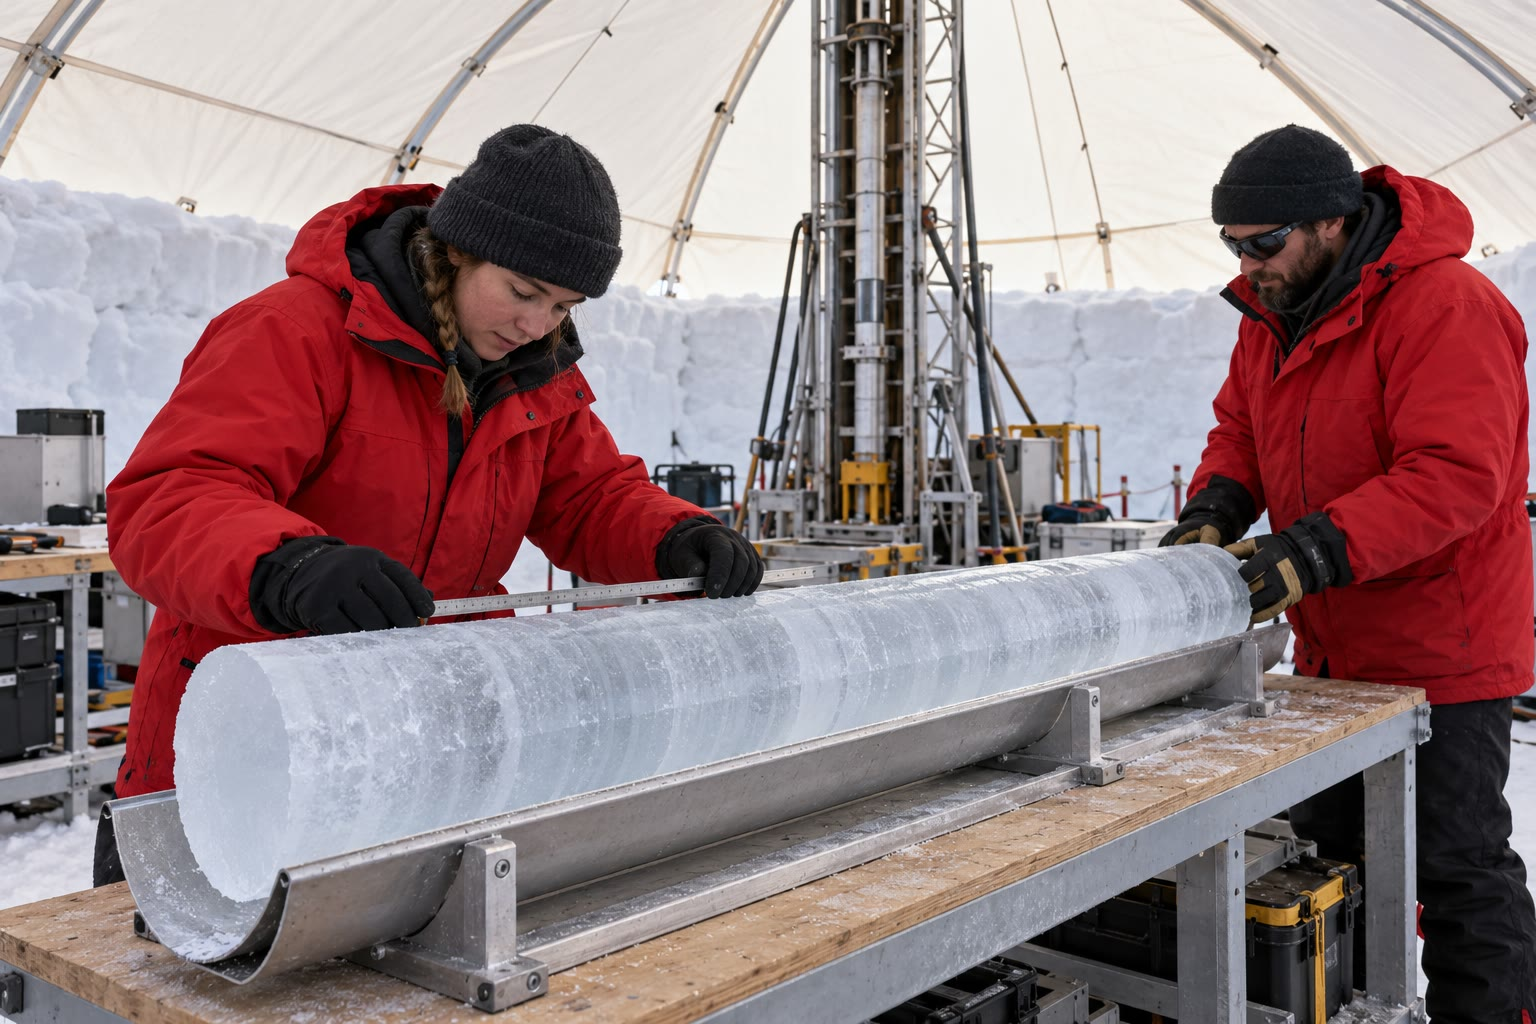
\includegraphics[width=\linewidth]{images/book5/ai/b3-ice-core-tent.jpg}

{\scriptsize Medição de um testemunho de gelo em um berço dentro de uma tenda de perfuração sobre um
manto de gelo, com a torre de perfuração ao fundo (Ilustração gerada por IA.)}
\end{minipage}
\end{inthelab}

\section{Exercícios}

\begin{exercise}[$\star$]\label{exo:b3:stable-isotopes:1}
Uma calcita tem $\delta^{18}\mathrm O = \qty{30.5}{\permil}$ e a água em que ela cresceu
tem \qty{-2.1}{\permil}, ambos em VSMOW. Calcule $\alpha$, $1000\ln\alpha$ e
$\Delta$. Quão distantes estão os dois últimos?
\end{exercise}

\begin{exercise}[$\star$]\label{exo:b3:stable-isotopes:2}
Uma estação costeira de alta latitude tem temperatura média anual de
\qty{-25}{\celsius}. Com as relações do capítulo para estações desse tipo,
preveja o $\delta^{18}\mathrm O$, o $\delta\mathrm D$ e o \omterm{def:b3:stable-isotopes:d-excess}{excesso de deutério} de sua
precipitação.
\end{exercise}
% ledger: dansgaard64:effects

\begin{exercise}[$\star$]\label{exo:b3:stable-isotopes:3}
Em uma bacia, os carbonatos têm $\delta^{13}\mathrm C = \qty{+1.0}{\permil}$ e a matéria
orgânica, \qty{-26.0}{\permil}. Com entradas em \qty{-5}{\permil}, calcule
$f_{\mathrm{org}}$.
\end{exercise}
% ledger: planavsky22:forg

\begin{exercise}[$\star$]\label{exo:b3:stable-isotopes:4}
Uma concha de braquiópode tem $\Delta_{47} = \qty{0.600}{\permil}$. Com a calibração
do capítulo, em que temperatura ela cresceu?
\end{exercise}
% ledger: isogeochem:d47

\begin{exercise}[$\star\star$]\label{exo:b3:stable-isotopes:5}
O vapor deixa o oceano com $\delta^{18}\mathrm O = \qty{-13}{\permil}$ e vai precipitando
com um $\alpha = 1.0100$ constante. Que fração dele resta quando o
vapor atinge \qty{-33}{\permil}? Qual é o $\delta^{18}\mathrm O$ da chuva
nesse ponto?
\end{exercise}
% ledger: white13c9:rayleigh

\begin{exercise}[$\star\star$]\label{exo:b3:stable-isotopes:6}
Neve com \qty{-40}{\permil} é comparada com água do oceano a 0. Calcule $\alpha$,
$1000\ln\alpha$, $1000(\alpha - 1)$ e $\Delta$ entre os dois. Qual das
aproximações da proposição falha, e em quanto?
\end{exercise}

\begin{exercise}[$\star\star$]\label{exo:b3:stable-isotopes:7}
Um foraminífero tem $\delta^{18}\mathrm O = \qty{+1.50}{\permil}$ em VPDB e cresceu em
água a \qty{0.00}{\permil} em VSMOW. Calcule sua temperatura de crescimento com o
método do capítulo, e quanto um erro de \qty{0.1}{\permil} no valor da
água altera-a.
\end{exercise}
% ledger: isogeochem:ko97

\begin{exercise}[$\star\star$]\label{exo:b3:stable-isotopes:8}
A pilha bentônica varia em \qty{1.77}{\permil} do presente até o último
máximo glacial. Remova a parcela de volume de gelo calculada no capítulo e
converta o restante em uma variação de temperatura da água profunda, usando a inclinação da
calibração da calcita perto de \qty{2}{\celsius}.
\end{exercise}
% ledger: data:lr04, white13c9:ice-volume, isogeochem:ko97

\begin{exercise}[$\star\star$]\label{exo:b3:stable-isotopes:9}
Uma pirita tem $\delta^{34}\mathrm S = \qty{10.0}{\permil}$ e $\delta^{33}\mathrm S =
\qty{8.2}{\permil}$. Calcule $\Delta^{33}\mathrm S$. O que isso diz sobre a
atmosfera quando a pirita se formou?
\end{exercise}
% ledger: white13c9:s-mif

\begin{exercise}[$\star\star\star$]\label{exo:b3:stable-isotopes:10}
Na condensação em sistema fechado, o vapor e todo o condensado formado permanecem
juntos em equilíbrio. Mostre que o vapor então tem $R_v/R_{v,0} = 1/[f +
\alpha(1 - f)]$, e compare-o com a \omterm{prop:b3:stable-isotopes:rayleigh-distillation}{destilação de Rayleigh} para $f = 0.2$ e
$\alpha = 1.01$.
\end{exercise}

\begin{exercise}[$\star\star\star$]\label{exo:b3:stable-isotopes:11}
A partir da estimativa de que \qty{2000}{Gt} de carbono de metano a
\qty{-60}{\permil} desloca o carbono trocável em \qty{-2.5}{\permil},
determine a massa do reservatório implícita, com $\delta_0 = 0$. Com essa massa, quanto
carbono orgânico a \qty{-25}{\permil} produz o mesmo deslocamento? Compare com a
faixa publicada.
\end{exercise}
% ledger: dickens11:petm

\begin{exercise}[$\star\star\star$]\label{exo:b3:stable-isotopes:12}
Mostre que, ao longo de uma trajetória de resfriamento, $\mathrm d\delta_v/\mathrm dT = (\alpha - 1)(1000 +
\delta_v)\,\mathrm d\ln e_s/\mathrm dT$. A \qty{-20}{\celsius}, onde o
vapor do modelo do capítulo tem $\delta^{18}\mathrm O = \qty{-49.1}{\permil}$
e a curva de sublimação fornece $\mathrm d\ln e_s/\mathrm dT =
\qty{0.0960}{K^{-1}}$, calcule esta inclinação.
\end{exercise}
% ledger: gkinis14:alpha-ice, iapws:melt-subl

\section{Problem: A jornada de uma gota de chuva até o Dome Ilse}

\begin{problem}[{Problema de fim de semana --- os isótopos da neve ao longo de um
percurso fictício, uma paleotemperatura e uma excursão isotópica do carbono}]\label{pb:b3:stable-isotopes:1}
Uma massa de ar deixa a borda de um manto de gelo fictício a \qty{0}{\celsius}
com vapor de $\delta^{18}\mathrm O = \qty{-20.0}{\permil}$ e $\delta\mathrm D =
\qty{-150}{\permil}$, e esfria sob pressão constante à medida que avança para o interior.
A neve se forma na estação Coast a \qty{-10}{\celsius}, em Midway a
\qty{-20}{\celsius} e em Dome Ilse a \qty{-30}{\celsius}, quando a fração
de vapor que resta é $f = 0.425$, $0.169$ e $0.0622$. Use os fatores de fracionamento gelo--vapor
do capítulo, constantes em cada trecho e iguais ao valor
correspondente à temperatura média do trecho.
% ledger: gkinis14:alpha-ice, iapws:melt-subl, dansgaard64:effects, isogeochem:ko97, isogeochem:d47, white13c9:ice-volume, data:lr04, planavsky22:forg, dickens11:petm

\medskip\noindent\textbf{Parte I --- Destilação.}
\begin{enumerate}
\item Calcule $\alpha^{18}$ e $\alpha^{\mathrm D}$ a $-5$, $-10$, $-15$, $-20$,
$-25$ e \qty{-30}{\celsius} (cinco algarismos significativos para oxigênio, quatro para
deutério).
\item Calcule o $\delta^{18}\mathrm O$ do vapor na chegada à estação Coast.
\item Calcule o da neve de Coast.
\item Repita para Midway (a razão de $f$ no trecho é $0.169/0.425$).
\item Repita para Dome Ilse.
\item Que fração do oxigênio-18 original do vapor ainda está no ar
em Dome Ilse?
\end{enumerate}

\medskip\noindent\textbf{Parte II --- Temperatura e deutério.}
\begin{enumerate}[resume]
\item Calcule a inclinação de $\delta^{18}\mathrm O$ da neve em função da
temperatura de condensação do Coast até Dome Ilse.
\item Qual temperatura média anual de superfície a relação das estações da
Groenlândia atribuiria à neve de Dome Ilse? Por que ela pode diferir de
\qty{-30}{\celsius}?
\item Calcule o $\delta\mathrm D$ da neve nas três estações da mesma maneira.
\item Calcule o \omterm{def:b3:stable-isotopes:d-excess}{excesso de deutério} delas. Como ele varia para o interior?
\item A neve de Dome Ilse está sobre a reta meteórica? O que o modelo
deixa de fora que a formação real da neve inclui?
\end{enumerate}

\medskip\noindent\textbf{Parte III --- Um foraminífero ao largo da costa.} Um
testemunho de sedimento ao largo da costa fornece foraminíferos bentônicos com \qty{3.25}{\permil}
VPDB no topo e \qty{5.02}{\permil} no último máximo glacial; a água de fundo
é \qty{0.00}{\permil} VSMOW hoje.
\begin{enumerate}[resume]
\item Calcule a temperatura atual da água de fundo com a
calibração da calcita.
\item Calcule a temperatura glacial supondo a água inalterada. O
resultado é possível?
\item Corrija a água glacial por uma queda do nível do mar de \qty{125}{m} e
recalcule. Qual é o resfriamento glacial da água de fundo?
\item Calcule o $\Delta_{47}$ esperado nas duas temperaturas e a
diferença entre elas.
\item Por que o termômetro de \omterm{def:b3:stable-isotopes:clumped}{isótopos agrupados} não precisa da
composição da água?
\end{enumerate}

\medskip\noindent\textbf{Parte IV --- Uma excursão de carbono.} Mais fundo no
testemunho, carbonatos com \qty{+0.5}{\permil} são interrompidos por uma breve
excursão de \qty{-3.0}{\permil}.
\begin{enumerate}[resume]
\item Antes da excursão, com $\delta_{\mathrm{in}} = \qty{-5}{\permil}$ e
$\Delta_B = \qty{-28}{\permil}$, calcule $f_{\mathrm{org}}$.
\item Tome o reservatório do exercício 11, \qty{46000}{Gt} em 0. Quanto carbono
a excursão exige se a fonte for metano a \qty{-60}{\permil}?
\item E se for carbono orgânico a \qty{-25}{\permil}?
\item E se for carbono do manto a \qty{-5}{\permil}?
\item Qual observação no mesmo testemunho poderia ajudar a escolher entre
as fontes?
\item Declare o $\delta^{18}\mathrm O$ da neve que cai em Dome Ilse.
\end{enumerate}
\end{problem}
